% Preambel
\documentclass[a4paper, 12pt]{article}
\title{Test {\LaTeX} Dokument}
\author{Håvard Solberg Nybøe}

% Pakker
% Språk
\usepackage[english, norsk]{babel} % Norsk språk
\usepackage{csquotes}
\usepackage{lipsum}
% Bibliografi
\usepackage[backend=biber, style=apa]{biblatex}
\addbibresource{bibliografi.bib}
\usepackage[hidelinks]{hyperref}
% Generelt
\usepackage[margin=1in]{geometry}
\usepackage{graphicx}
\usepackage{import}

\setlength{\parindent}{0em}
\setlength{\parskip}{.8em}

% Innhold
\begin{document}

\pagenumbering{roman} % Sidenummerering for forord og toc

\import{./}{title}
\newpage

% innholdsfortegnelse
\tableofcontents
\listoffigures
\listoftables
\newpage

\pagenumbering{arabic} % Sidenummerering for resten av dokumentet

\import{sections}{sammendrag}
\import{sections}{innledning}
\import{sections}{bakgrunn}
\import{sections}{teori}
\import{sections}{metode}
\import{sections}{resultater}
\import{sections}{analyse}
\import{sections}{diskusjon}
\import{sections}{konklusjon}

\section{Test}
\subsection{Test test}
Dette er en test

Dette er enda en test

    Hei \parencite{druckmann2020}\\
    Hei \parencite{druckmann2013}\\
    Hei \parencite{druckmann2014}
    
    \begin{figure}[h]\label{r/place}
        \centering
        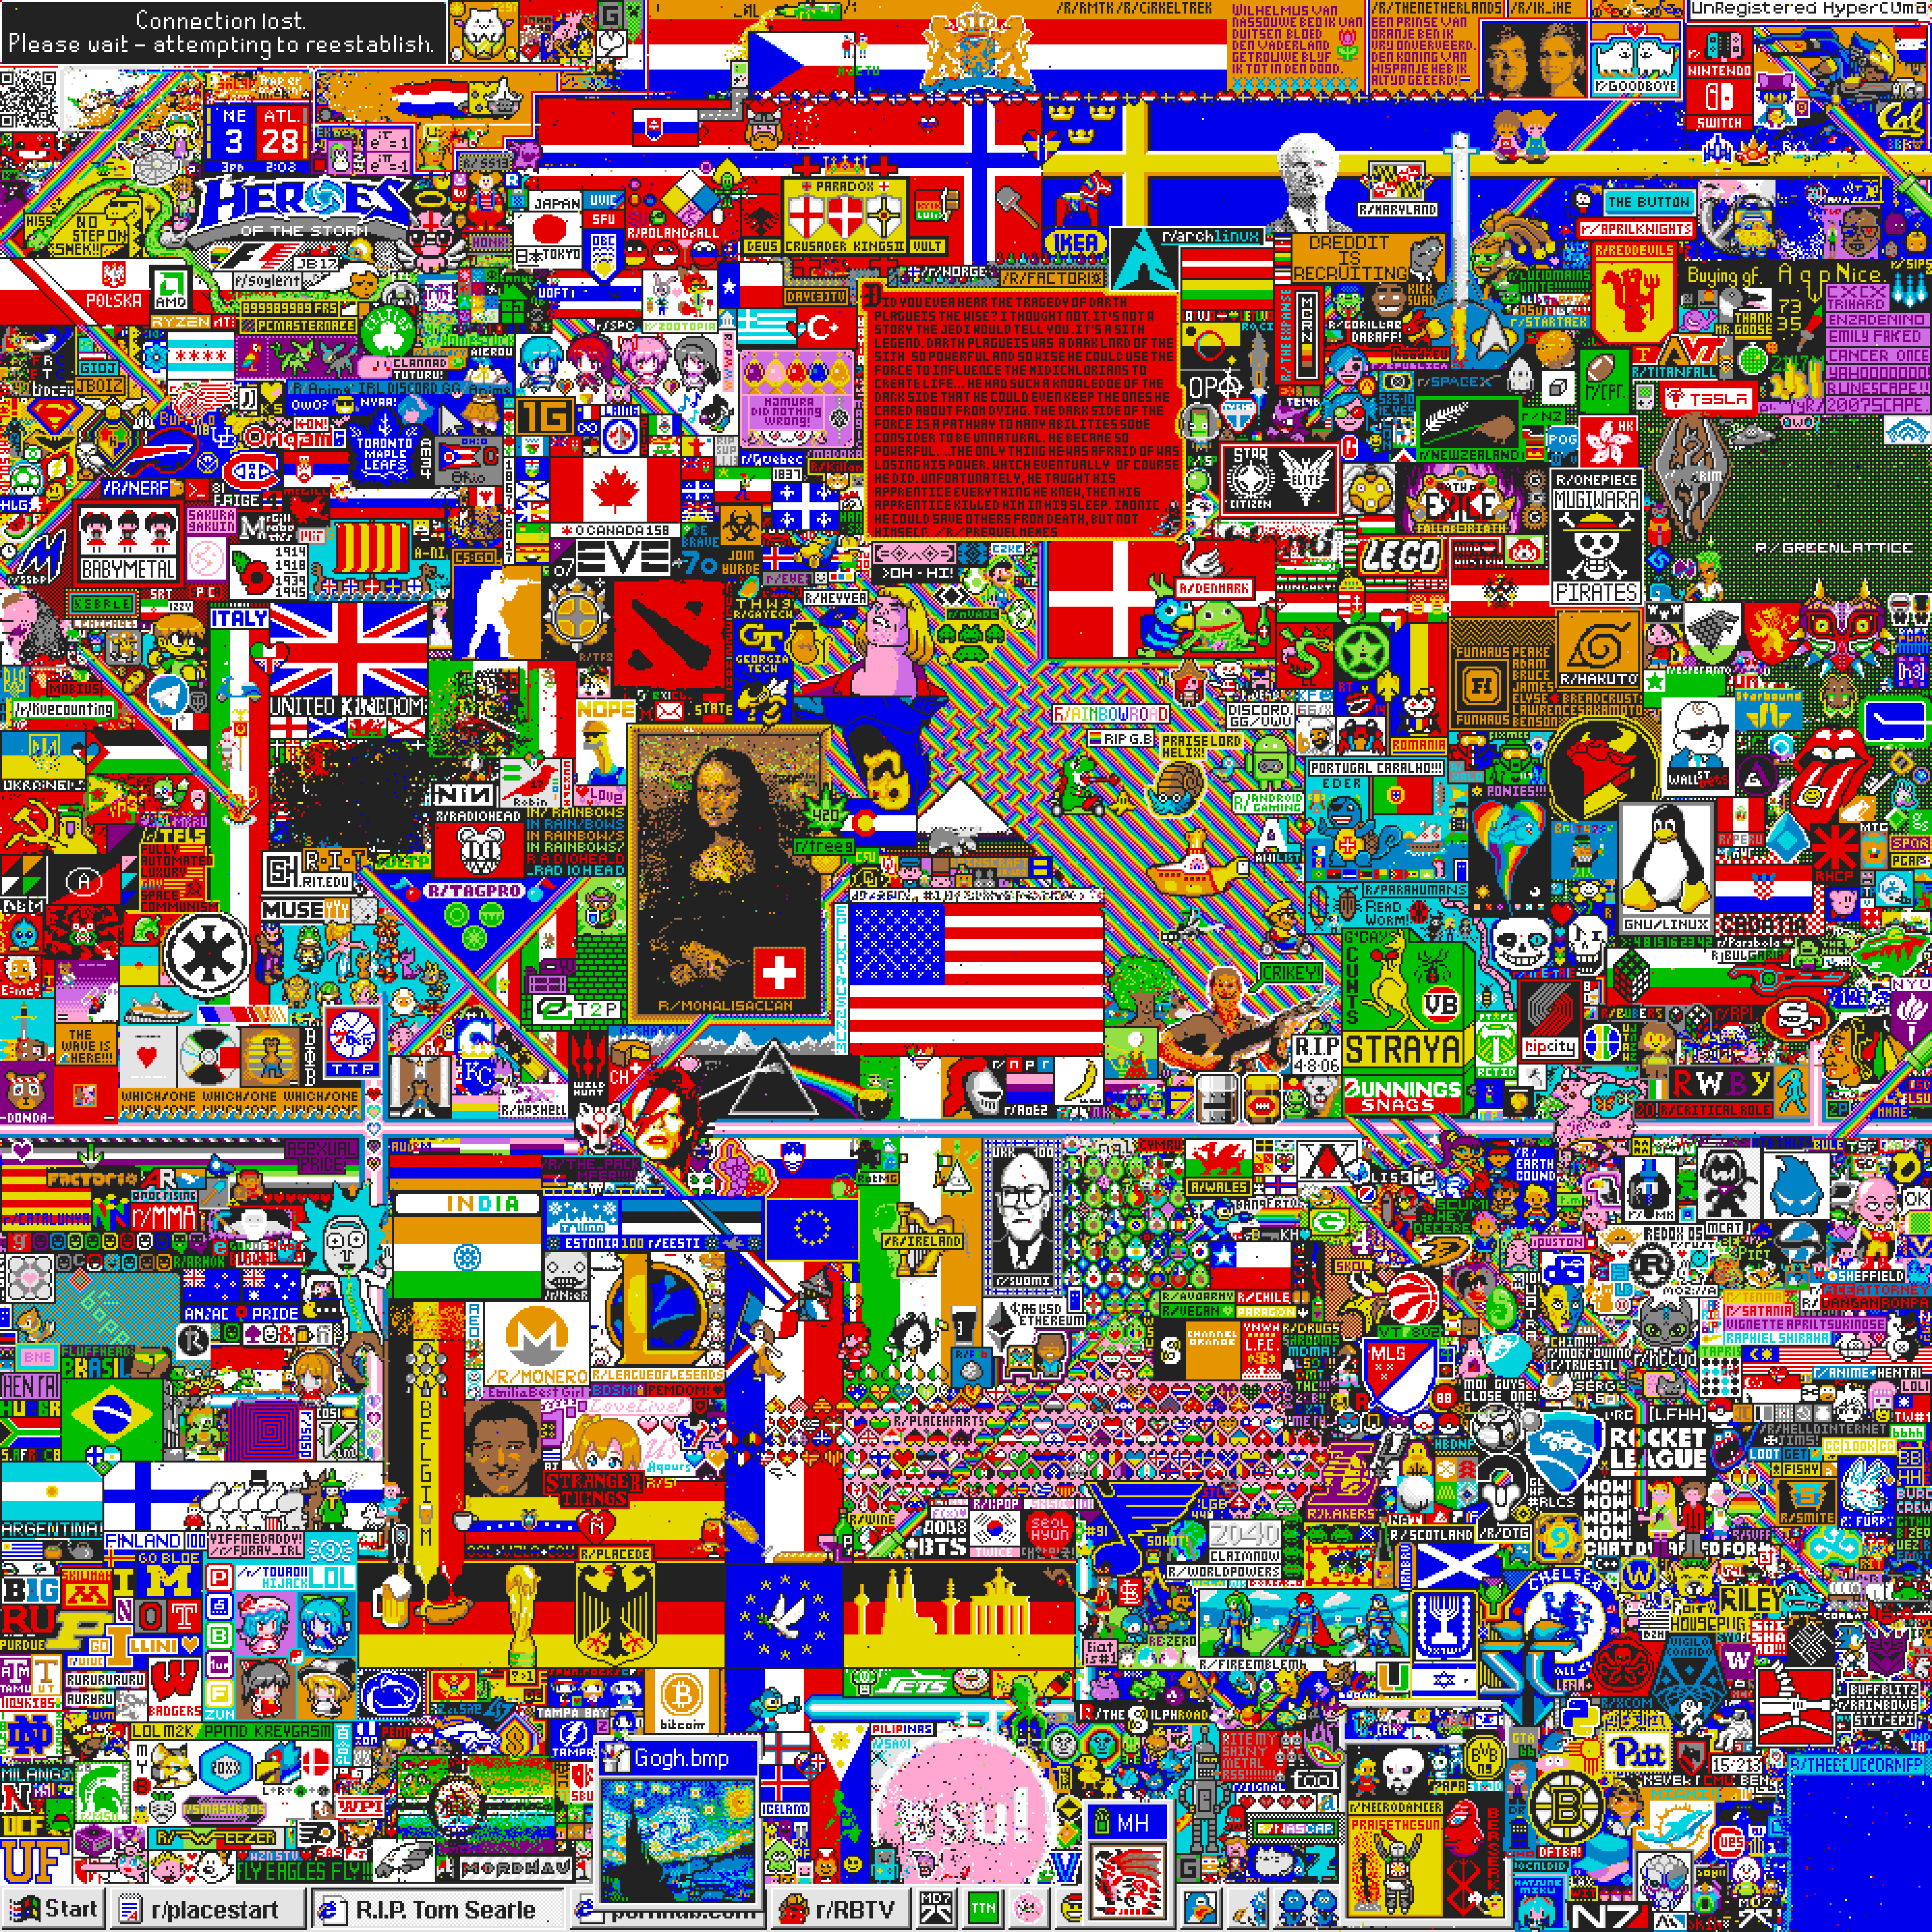
\includegraphics[width=.6\textwidth]{img/r_place.png}
        \caption{Kunstverk laget av r/place.}
    \end{figure}
    
    %% BIBLIOGRAFI %%
    \newpage
    \printbibliography[heading=bibintoc]
    

\end{document}
